%%%%%%%%%%%%%%%%%%%%%%%%%%%%%%%%%%%%%%%%%%%%%%%%%%

\chapter{Cálculo y Análisis.}

%%%%%%%%%%%%%%%%%%%%%%%%%%%%%%%%%%%%%%%%%%%%%%%%%%

Este capítulo trata de todas las funciones dentro de la biblioteca
relacionadas con el cálculo infinitesimal y el análisis matemático.
Matlab no es un lenguaje de cálculo simbólico, no calcula ni derivadas
ni primitivas. Todas las rutinas de este capítulo están enfocadas
al cálculo numérico.


\section{Funciones elementales.}

Ya hemos comentado que Matlab posee una importante biblioteca de funciones,
es el momento de conocerla con un poco más de detalle


\section{Polinomios}

En Matlab los polinomios se almacenan como vectores de coeficientes.
Cada componente del vector es un coeficiente ordenado del término de
mayor a menor orden. La manera más habitual de iniciar un polinomio es
utilizar la siguiente función:

\begin{description}
\item [poly\texttt{\index{poly}}]Inicia un polinomio. Si el argumento
  es una matriz cuadrada devuelve el polinomio característico, si es
  un vector devuelve un polinomio cuyas raíces son los elementos del
  vector.
\end{description}
También nos serán muy útiles las funciónes:

\begin{description}
\item [roots\texttt{\index{roots}}]Devuelve las raíces del polinomio
  cuyos coeficientes son los elementos del vector argumento.
\item [polyval\texttt{\index{polyval}}]Calcula el valor del polinomio
  en el punto dado
\item [polyout\texttt{\index{polyout}}](Octave) Escribe un polinomio
  en un formato más leíble:
\end{description}
Por ejemplo, si queremos escribir el polinomio
$s^{5}-8s^{4}+3s^{2}+16$:

\begin{verbatim}
>> polinomio = [1,-8,0,+3,0,16]
>> polyval(polinomio,44)
ans= 134937280
\end{verbatim}
Los polinomios se pueden manipular analíticamente con las siguientes
funciones:

\begin{description}
\item [polyder\texttt{\index{polyder}}]Deriva un polinomio.
\item [polyint\texttt{\index{polyint}}]Integra analíticamente un
  polinomio.
\item [conv\index{conv}]Multiplica dos polinomios.
\item [deconv\index{deconv}]Dados dos polinomios $a$ e $y$ halla $b$ y
  $r$ que cumplen:\[ y=(a*b)+r\]

\item [residue\index{residue}]Descompone el cociente de dos polinomios
  en fracciones con un único polo. Por ejemplo, dados los polinomios
  $p=s^{2}+s+1$ y $q=s^{3}-5s^{2}+8s-4$ la descomposición sería:

$$\frac{s^{2}+s+1}{s^{3}-5s^{2}+8s-4}=
\frac{-2}{s-2}+\frac{7}{(s-2)^{2}}+\frac{3}{s-1}$$

\end{description}

\subsection{Evaluación de
  funciones.\label{sub:Evaluaci=F3n-de-funciones.}}

Los polinomios son una parte importantísima del cálculo numérico
porque son su nexo fundamental con el cálculo simbólico. Uno de los
elementos fundamentales en el cálculo numérico es la aproximación de
una función analítica por otra con una expresión numérica lo más
equivalente posible.  Todas las funciones analíticas no existen
realmente dentro de un programa de cálculo numérico por limitaciones
del propio ordenador; la aritmética exacta es algo prohibitivo. La
evaluación de funciones se realiza por series de potencias almacenadas
por sus coeficientes; este es el funcionamiento de la evaluación de
cualquier función analítica en un programa de cálculo numérico. Las
series de potencias acotan el error con el número de términos y el
orden de la serie; a mayor precisión más términos a evaluar. Por
ejemplo, si Matlab quiere obtener el valor de la función seno en un
punto evaluará la serie:

$$\sin x=\sum_{k=0}^{\infty}\frac{(-1)^{k}}{(2k+1)!}x^{2k+1}$$

O si quiere evaluar la función de Bessel de primera especie:

$$J_{n}(x)=\left(\frac{x}{2}\right)^{n}\sum_{k=0}^{\infty}
\frac{(-\frac{1}{4}x^{2})^{k}}{k!(k+n)!}$$

Si este es el funcionamiento interno de Matlab será muy beneficioso
que tengamos esto en cuenta cada vez que tengamos que evaluar
funciones especialmente pesadas. No necesitamos aritmética exacta,
evaluar una precisión mayor a la de la máquina es malgastar recursos.

Supongamos que tenemos una función con una gran cantidad de funciones
trigonométricas. Es probable que alguna vez en nuestra vida tengamos
funciones de dos y tres líneas de código. Evaluarla entera es una
pérdida de recursos. Imaginemos además que estemos integrando una
ecuación diferencial cuyo término es esta misma función. Evaluando
todos los términos no estamos ganando precisión; estamos sumando y
restando polinomios de un orden mayor al que queremos con valores que
se cancelan continuamente. Utilizando la interpolación polinómica
podemos acelerar cualquier código hasta en un órden de magnitud.


\section{Derivadas\index{Derivadas}}

Todas las funciones de este apartado se refieren a la derivada
numérica.  No son derivadas de una función analítica sino el resultado
de aplicar las ecuaciones de diferencias de orden enésimo a una serie
discreta de puntos.

\begin{description}
\item [diff\texttt{\index{diff}}]Aplica la fórmula de diferencias
  enésimas a una serie de puntos
\item [gradient\texttt{\index{gradient}}]Calcula el gradiente numérico
  de una matriz. Esta función es muy interesante por su relación
  íntima con la función \texttt{quiver}. Si queremos expresar un
  determinado campo vectorial a partir de su función potencial, siendo
  el potencial la función $\phi(x,y)$ entonces el campo es en cada
  punto $\left(\partial_{x}\phi,\partial_{y}\phi\right)$, es decir,
  $\nabla\phi$. Para pintar este campo vectorial sólo tenemos que
  hacer \texttt{quiver(gradient(phi)) .}
\end{description}

\section{Integrales\index{Integrales}}

La integración es un vasto campo del cálculo numérico y así
se refleja en Matlab. Podemos hacer tanto integrales en una dimensión
como en dos. Las rutinas más relevantes son:

\begin{description}
\item [quad\texttt{\index{quad}}]Integración numérica de una función
\item [quadl\texttt{\index{quadl}}]Su uso es idéntico que la función
  anterior pero contiene un algoritmo de cuadratura de mayor
  precisión.
\item [dblquad\texttt{\index{dblquad}}] Calcula la integral
  doble de una función de dos variables. \texttt{quad2dc\index{quad2dc}}
  y \texttt{quad2dg\index{quad2dg}} en Octave.  En el primer caso
  utiliza una cuadratura de Gauss-Chebyshev y en el segundo utiliza un
  esquema de integración de Gauss.
\item [triplequad\texttt{\index{triplequad}}]No existe aún en Octave.
  Calcula la integral de volúmen de una función de tres variables.
\item [trapz\texttt{\index{trapz}}]Aplica la regla del trapecio para
  calcular la integral numérica de una serie discreta de puntos.
\end{description}

El único misterio que puede tener la integración numérica es cómo
pasar la función a integrar como argumento.  La manera recomendada de
hacerlo es, como siempre en el que una función sea un argumento, con
un function handle o una función anónima.

Por ejemplo, para calcular esta integral:

\[  \int_o^{2\pi} \sin(x)\cos(pi)\ dx\]

utilizaremos el código siguiente:

\begin{verbatim}
>> quad(@(x) sin(x)*cos(x),0,2*pi)
\end{verbatim}

Difícilmente encontraremos un caso en el que, teniendo la forma de la
función analitica, sea necesario más que una función anónima.  Las
dudas llegan cuando se quiere integrar una serie de datos y no se
dispone de ninguna función.

Si disponemos de una serie de datos unidimensional $(x,y)$ uno puede
acudir directamente a la regla del trapecio.  Podemos utilizar una
interpolación con splines para llegar hasta orden 3 en la
integración. El truco es crear una función anónima que llame a la
interpolación como sigue:

\begin{verbatim}
>> x=1:10;y=rand(1,10);
>> f=@(x1) interp1(x,y,x1);
>> quad(f,1,10)
ans =  3.9732
\end{verbatim}

Es muy sencillo demostrar que utilizar esta técnica en una dimensión
no es necesario

\begin{verbatim}
>> format long
>> quad(f,1,10)
ans =  3.9732
>> trapz(x,y)
ans =  3.9732
\end{verbatim}

Donde sí es útil es cuando se quiere integrar una superficie que no se
ha definido analíticamente sino que se dispone de una serie de puntos
de la forma $(x,y,z)$.  Distinguiremos dos casos según cómo se ordenen
los datos

\begin{itemize}
\item Si los datos están ordenados en una malla estructurada puede
  utilizarse \texttt{interp2} para generar la función.
\item Si los datos no obedecen a ningún orden la interpolación se hará
  con la función \texttt{griddata}
\end{itemize}

Un ejemplo del segundo caso puede ser el siguiente:

\begin{verbatim}
pending
\end{verbatim}

En este caso hay que recordar que Matlab y Octave utilizan métodos
funciones y algoritmos completamente distintos para la
integral. Mientras Matlab parece que reduce el problema a una serie de
integrales en una dimensión Octave utiliza fórmulas de cuadratura en
dos dimensiones. Las funcoines tienen nombres distintos (no hay
ninguna \texttt{dblquad} en Octave) para que los usuarios san
conscientes de esta diferencia.\footnote{Los algoritmos de integración
por cuadratura numérica escalan mal con el número de dimensiones a
integrar.  En el caso de funciones de muchas dimensiones es más
eficiente utilizar la integración Montecarlo.}

Este tipo de cálculos son especialemente lentos, el porqué es bien
sencillo.  Una de las operaciones más lentas en Matlab en comparación
con otros lenguajes de programación es la llamada a una función.  Si
se integra con matrices que contengan más de miles de puntos puede ser
que exista un problema de rendimiento.  En este caso es recomendable,
antes de quizás escribirse un algoritmo de integración propio,
modificar el parámetro de error máximo o reducir el orden de la
interpolación de cúbico (splines) a lineal.

\subsection{Integración en dos dimensiones.  Diferencias entre Matlab
  y Octave}

\section{Ecuaciones diferenciales\index{ecuaciones diferenciales} ordinarias.}

Se podría decir que hay un método de integración para cada problema.
Existen multitud de esquemas de integración y escoger uno de ellos
no es fácil. Uno de los objetivos de las funciones de Matlab es intentar
ser lo más universales posible. La función perfecta sería la que sin
configuración alguna integrara cualquier EDO\index{EDO} con una precisión
aceptable; desgraciadamente no existe y probablemente no exista nunca.

Una consideración esencial antes intentar resolver una EDO es saber
si el paso temporal viene condicionado por la precisión numérica o
por criterios de estabilidad. El segundo caso es bastante más preocupante
que el primero. Cuando la función introduce gradientes elevados que
acortan significativamente el paso de la iteración se dice que el
problema es \emph{stiff}\index{stiff}. En estos casos será apropiado
utilizar un esquema de integración implícito que a costa de mayor
coste computacional por paso permite llegar al resultado con muchas
menos iteraciones. Saber si un problema es stiff o no es tan laborioso
o más que resolverlo. Para saber si utilizar un esquema explícito
o implícito la estrategia será la siguiente:

\begin{enumerate}
\item Represenataremos la función a integrar para comprobar si tiene discontinuidades
o gradientes muy elevados
\item Si no tiene ninguna singularidad utilizaremos un esquema explícito
(no stiff) calculando el tiempo de proceso.
\item Si el tiempo nos parece demasiado elevado cambiaremos a un esquema
implícito
\item Si el tiempo sigue siendo demasiado elevado y la programación es correcta
puede ser que la función sea demasiado costosa de evaluar. Para solucionarlo
escribiremos la función en otro lenguaje de programación como C, C++
o Fortran y la convertiremos en un archivo que Matlab entienda.
\end{enumerate}
La precisión numérica es también muy importante pero el mismo esquema
de integración es capaz de controlarla. Daremos como válido que a
mayor precisión numérica mayor dificultad para obtener una solución
estable.

Las diferencias entre Matlab y Octave en este caso son más que significativas.
Octave dispone de las funciones de integración de Matlab pero existen
sólo por motivos de compatibilidad, son mucho más lentas y no se pueden
configurar. Sin embargo Octave integra la suite ODEPACK\index{ODEPACK},
uno de los paquetes de integración de EDOs más robusto y efectivo.


\subsection{Octave}

Octave cuenta con las funciones de integración de Matlab pero están
programadas como archivos \texttt{.m} y no como parte de una
biblioteca binaria. Es muy recomendable que utilcemos la función
\texttt{lsode} (Livermore Solver for Ordinary Differential Equations),
parte de ODEPACK.  Utiliza un método multipaso Adams Para problemas no
stiff y una BDF\index{BDF} (Backward Differentiation Formula) para los
problemas stiff.%
\footnote{Personalmente creo que éste es uno de los pocos casos en el
  que Octave es superior a Matlab. Ni entiendo ni comparto la
  organización de las rutinas de integración de Matlab, me parece
  confusa, desacertada y poco óptima.%
}

\begin{description}
\item [lsode\index{lsode}](Octave) Es el driver general de integración
  de ecuaciones diferenciales ordinarias.
\end{description}
\begin{verbatim} [X, ISTATE, MSG] = lsode (FCN, X_0, T, T_CRIT)
\end{verbatim}
Resuelve el problema de Cauchy de la forma:
$$ \frac{dy}{dt}=f(x,t)$$
dadas las condiciones iniciales.

\begin{description}
\item [\texttt{FCN}]Matriz de dos elementos tipo cadena de caracteres.
  El primero es el nombre de la función que queremos integrar y el
  segundo la función que calcula el jacobiano.
\end{description}
La función a integrar debe definirse necesariamente mediante una
función, ya sea dentro del script o en un archivo a parte. La cabecera
tendrá sólo dos variables y su forma será

\begin{verbatim}
XDOT=FUNC(X,T)
\end{verbatim}
donde tanto \texttt{X} como \texttt{XDOT} pueden ser escalares o
vectores.  El jacobiano también tendrá la forma
\begin{verbatim}
JAC=FJAC(X,T)
\end{verbatim}
donde \texttt{JAC} será la matriz que implemente las funciones
derivadas parciales según el orden establecido por la variable
\texttt{X}. Se usa para acelerar la integración en problemas stiff.

\begin{description}
\item [\texttt{X\_0}]Vector de condiciones iniciales.
\item [\texttt{T}]Vector que determina los instantes temporales en los
  que se dará una solución.
\item [\texttt{T\_CRIT}]Puntos en los que la rutina no debe integrar
  por la existencia de singularidades.
\item [\texttt{X}]Vector de soluciones en los instantes \texttt{T}
\end{description}
Si la integración no ha sido satisfactoria \texttt{ISTATE} devolverá
el valor 2 y \texttt{MSG} nos dará más información.

\begin{description}
\item [lsode\_options]Función de configuración de \texttt{lsode}
\end{description}
\begin{verbatim}
lsode_options index{lsode options} (OPT, VAL)
\end{verbatim}
Llamada con un único argumento (\texttt{OPT}) nos dirá el valor de la
opción de configuración que hayamos solicitado. Pasando dos argumentos
podremos cambiarlos. Las opciones disponibles son los de la tabla
siguiente:

%
\begin{table}[H]
  \centering{}\begin{tabular}{|c|m{8cm}|p{3cm}|}
    \hline 
    Parámetro de configuración&
    Valores admitidos&
    Valor por defecto\tabularnewline
    \hline
    \hline 
    \texttt{'absolute tolerance'}&
    Error absoluto para cada caso de integración. Un escalar o un vector
    cuyo tamaño debe ser el mismo que el número de puntos a calcular&
    $1.4901\times10^{-8}$\tabularnewline
    \hline 
    \texttt{'relative tolerance'}&
    Error relativo permitido para cada paso de integración. Es un escalar&
    $1.4901\times10^{-8}$\tabularnewline
    \hline 
    \texttt{'integration method'}&
    \texttt{'adams'} o \texttt{'non-stiff'} para un esquema explícito
    o \texttt{'bdf'} o \texttt{'stiff'} para un esquema implícito&
    \texttt{'stiff'}\tabularnewline
    \hline 
    \texttt{'initial step size'}&
    El valor del primer paso de integración. Es un escalar&
    automático\tabularnewline
    \hline 
    \texttt{'maximum order'}&
    Un número del 1 al 12 para \texttt{'non-stiff'} y del 1 al 5 para
    \texttt{'stiff'}&
    Órdenes máximos\tabularnewline
    \hline 
    \texttt{'minimum step size'}&
    Paso de integración mínimo. Un escalar&
    0\tabularnewline
    \hline 
    \texttt{'step limit'}&
    Máximo número de iteraciones admitidas.&
    100000\tabularnewline
    \hline
  \end{tabular}


  \caption{Valores de configuración de \texttt{lsode\_options}}
\end{table}


Pronto veremos un ejemplo de cómo usar esta función.


\subsection{Matlab}

El planteamiento de las rutinas para ODEs de Matlab es completamente
distinto. En vez de tener una función que sirve más o menos para todo
nos permite escojer el método de integración. Disponemos de los presentes
en la tabla \ref{cap:Funciones-de-integraci=F3n}:

%
\begin{table}[H]
\centering{}\begin{tabular}{|m{2cm}|>{\centering}m{3cm}|>{\raggedright}p{10cm}|}
\hline 
Función&
Tipo de problema&
Observaciones\tabularnewline
\hline
\hline 
\texttt{ode45\index{ode45}}&
no stiff&
Esquema Runge Kutta (4,5). Debe ser la primera opción\tabularnewline
\hline 
\texttt{ode23\index{ode23}}&
no stiff&
Esquema Runge Kutta de menor orden. Mayor estabilidad que \texttt{ode45}.\tabularnewline
\hline 
\texttt{ode113\index{ode113}}&
no stiff&
Método multipaso de mayor precisión\tabularnewline
\hline 
\texttt{ode15s\index{ode15s}}&
stiff&
Para problemas stiff.\tabularnewline
\hline 
\texttt{ode15i\index{ode15i}}&
stiff&
Método completamente implícito. Lo usaremos en casos puntuales\tabularnewline
\hline 
\texttt{ode23s\index{ode23s}}&
stiff&
Primera opción para problemas stiff.\tabularnewline
\hline 
\texttt{ode23t\index{ode23t}}&
no stiff/stiff&
-\tabularnewline
\hline 
\texttt{ode23tb\index{ode23tb}}&
stiff&
-\tabularnewline
\hline
\end{tabular}


\caption{\label{cap:Funciones-de-integraci=F3n}Funciones de integración de
EDOs de Matlab}
\end{table}


La llamada básica es la misma para todas ellas y tiene la forma:

  \begin{verbatim}
[T,Y] = solver(odefun,tspan,y0)

[T,Y] = solver(odefun,tspan,y0,options)

[T,Y,TE,YE,IE] = solver(odefun,tspan,y0,options)
 \end{verbatim}
\texttt{odefun} es la llamada convencional a una función, preferiblemente
un function handle. A diferencia de \texttt{lsode} la función debe
tener la forma:
$$\frac{dy}{dt}=F(t,x)$$
y su resultado \textbf{debe ser un vector columna}. \texttt{tspan}
es un vector de dos componentes con el tiempo inicial y final de integración;
finalmente \texttt{y0} es el vector con la condición inicial. Los
parámetros de salida son los usuales, \texttt{T} e \texttt{Y} son
respectivamente los vectores tiempo y solución del problema. En breve
propondremos un ejemplo

También es necesario que conozcamos la función de configuración \texttt{odeset}.
La cantidad de opciones es bastante mayor a las disponibles en \texttt{lsode}
de modo que lo más sensato será consultar la ayuda.


\subsection{Solución de la ecuación de Van der Pol\index{Van der Pol}}

La ecuación diferencial de Van der Pol es:
$$ mx^{\prime\prime}-\alpha
x^{\prime}+\beta\left(x^{\prime}\right)^{3}+kx=0$$
 No es más que el
movimiento de una masa oscilante con amortiguamiento lineal y no
lineal a la vez. Adimensionalizando el problema llegamos a la
ecuación.

$$x^{\prime\prime}+x+\mu(x^{\prime2}-1)x^{\prime}=0$$
 Esta ecuación
tiene la particularidad de que a medida que el parámetro $\mu$ aumenta
el problema se vuelve stiff. Con un $\mu$ de orden unidad el sistema
puede considerarse no stiff mientras que si aumenta hasta ser del
orden del millar la ecuación introduce gradientes muy acusados. Este
comportamiento tan particular la hace perfecta para ensayar los
distintos métodos de integración. Lo primero es descomponer la
ecuación en un problema que Matlab pueda entender:

$$
\begin{array}{l}
  \frac{dy_{1}}{dt}=y_{2}\\
  \frac{dy_{2}}{dt}=\mu y_{2}(1-y_{1}^{2})-y_{1}\end{array}$$
con condiciones de contorno $y_{1}(0)=2$ e $y_{:2}(0)=0$. Resolveremos
el problema para $\mu=1$ y $\mu=1000$ porque Matlab ya cuenta con
estas funciones (\texttt{vdp1} y \texttt{vdp1000}). Para agilizar
los cálculos escribiremos las funciones para Octave en C++:

\begin{verbatim}
#include <octave/oct.h>
DEFUN_DLD (vdp1,args, ,
            "Ecuacion de Van der Pol para mu=1 ")
{
  ColumnVector xdot (2);
  ColumnVector x (args(0).vector_value());
  float mu=1;
  xdot(0) = x(1);
  xdot(1) = mu*x(1)*(1-x(0)*x(0))-x(0);
  return octave_value (xdot);
}
\end{verbatim}
Y la función para $\mu=1000$:

  \begin{verbatim}
#include <octave/oct.h>
DEFUN_DLD (vdp1000,args, ,
            "Ecuacion de Van der Pol para mu=1000 ")
{
  ColumnVector xdot (2);
  ColumnVector x (args(0).vector_value());
  float mu=1000;
  xdot(0) = x(1);  
  xdot(1) = mu*x(1)*(1-x(0)*x(0))-x(0);
  return octave_value (xdot);
}
\end{verbatim}

\subsubsection{Integración del problema no stiff (\texttt{vdp1}\index{vdp1})}

Integrar un problema no stiff es mucho más sencillo que un problema
stiff. La inestabilidad numérica tiene efectos mucho más importantes
que la pérdida de precisión. Los esquemas de integración que manejaremos
son de paso variable. Esto significa que la propia subrutina calcula
el paso de integración para, sea cual sea la función y el esquema
utilizado, el resultado sea numéricamente correcto.

\begin{itemize}
\item Octave
\end{itemize}
  \begin{verbatim}
>> lsode_options('integration method','non-stiff')
>> y=lsode('vdp1',[0 2],linspace(0,20,1000));
 \end{verbatim}
\begin{itemize}
\item Matlab
\end{itemize}
  \begin{verbatim}
>> [tout,xout]=ode45(@vdp1,[0 20],[2 0]); 
 \end{verbatim}
La diferencia esencial entre Octave y Matlab es que el primero pide
por defecto los puntos en los que queremos la solución. Matlab prefiere
resolver el problema y dar los puntos en el tiempo en los que se ha
pasado durante la integración. Es por ese motivo por el que el argumento
{}``tiempo'' es en el primer caso un vector de un millar de elementos
mientras que en el segundo es tan solo un par de escalares.

La superposición de ambas soluciones es un ejemplo perfecto para ver
trabajar los esquemas de paso variable. Apreciamos en la figura \ref{cap:odenostiff}
que el paso de integración disminuye según la curvatura de la solución

%
\begin{figure}[h]
\centering{}

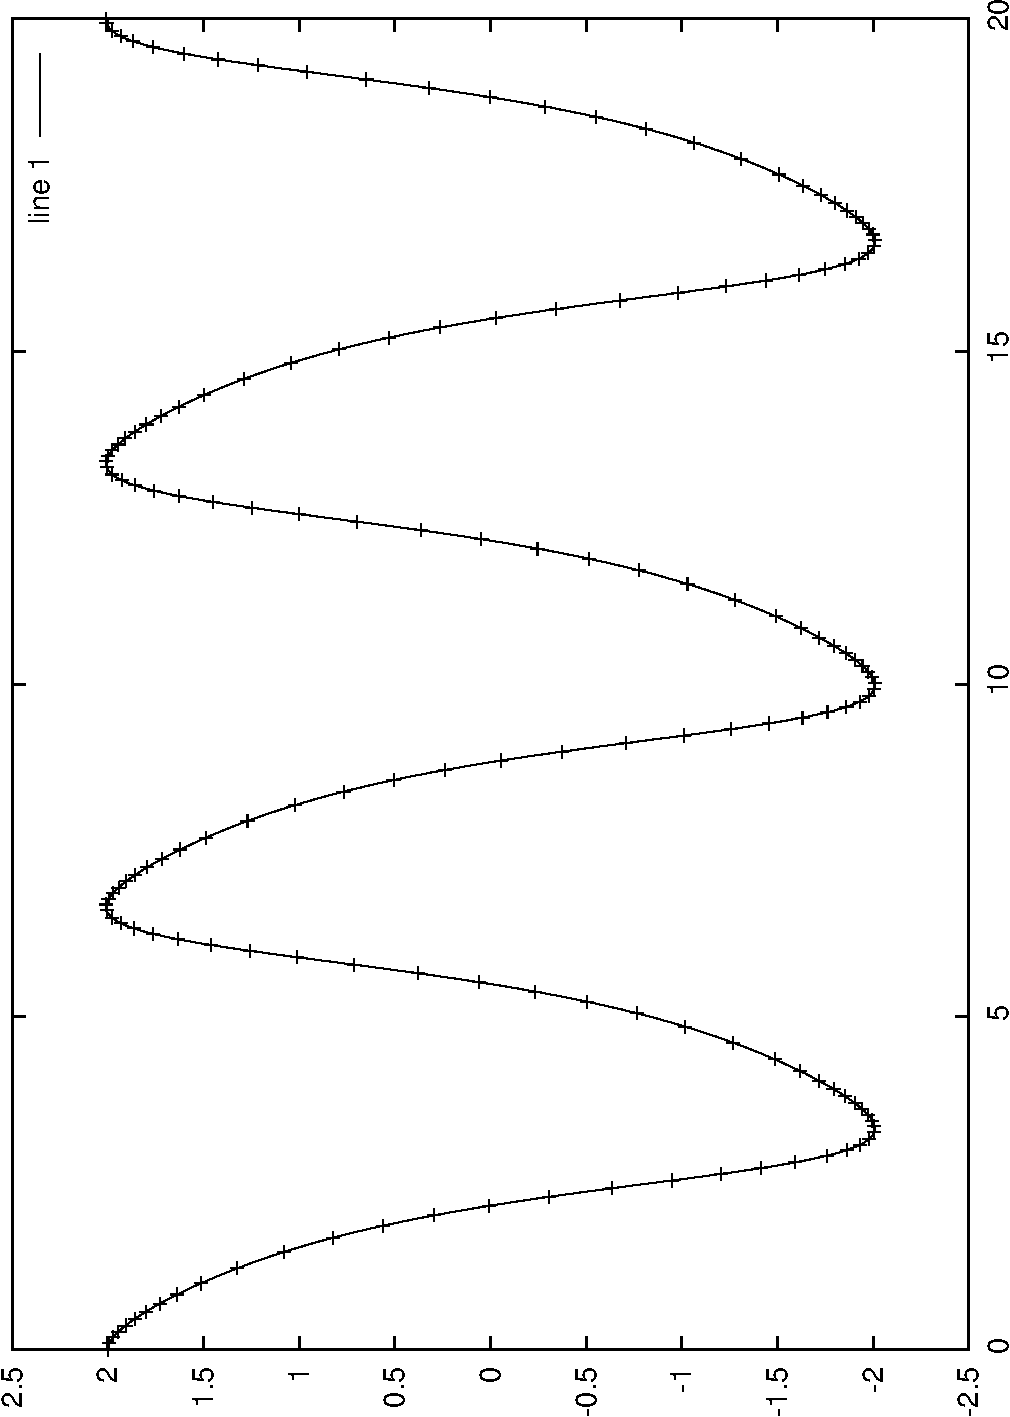
\includegraphics[%
  height=11cm,
  keepaspectratio,
  angle=-90]{figuras/comparisonode}


\caption{\label{cap:odenostiff}Solución de la ecuación de Van der Pol con
$\mu=1$}
\end{figure}



\subsubsection{Integración del problema stiff (\texttt{vdp1000}\index{vdp1000})}

Como los problemas stiff introducen gradientes elevados en la solución
el paso de integración de un esquema explícito se va haciendo tan
pequeño que su avance es demasiado corto. Es precisamente lo que ensayamos
en este caso. Si intentamos resolver la ecuación de Van der Pol con
$\mu=1000$ y $t\in[0,3000]$ mediante un esquema explícito:

\begin{itemize}
\item Octave
\end{itemize}
  \begin{verbatim}
>> lsode_options('integration method','non-stiff')

>> y=lsode('vdp1000',[0 2],linspace(0,3000,100000));
 \end{verbatim}
\begin{itemize}
\item Matlab
\end{itemize}
  \begin{verbatim}
>> [tout,xout]=ode45(@vdp1000,[0 3000],[2 0]); 
 \end{verbatim}
nos encontramos con la desagradable sorpresa de que el calculo no
termina nunca. Esto es porque la solución, aunque es regular, tiene
puntos con gradiente casi infinito.

La solución es utilizar un esquema implícito o semimplícito. Por ejemplo:

\begin{itemize}
\item Octave
\end{itemize}
  \begin{verbatim}
>> lsode_options('integration method','stiff')

>> ystiff=lsode('vdp1000',[2 0],linspace(0,20,1000));
 \end{verbatim}
\begin{itemize}
\item Matlab
\end{itemize}
  \begin{verbatim}
>> [tout,xout]=ode23s(@vdp1000,[0 3000],[2 0]);
 \end{verbatim}
Efectivamente, la solución demuestra por qué el problema es stiff
(Figura \ref{cap:odestiff}):

%
\begin{figure}[H]
\centering{}

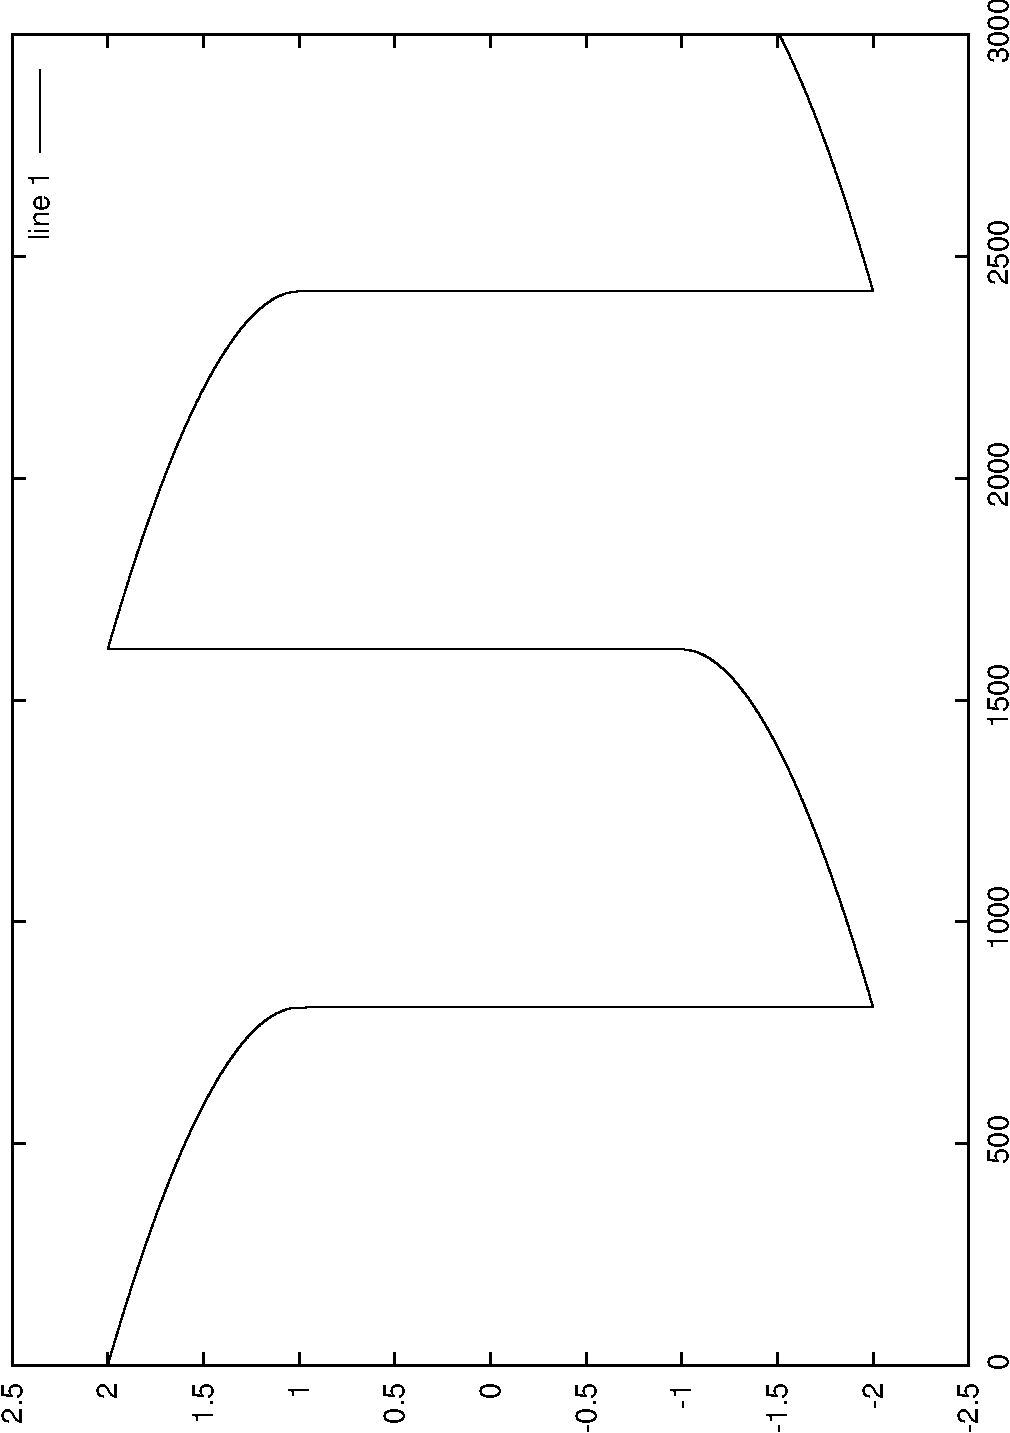
\includegraphics[%
  height=11cm,
  keepaspectratio,
  angle=-90]{figuras/comparisonodestiff}


\caption{\label{cap:odestiff}Solución de la ecuación de Van der Pol con $\mu=1000$}
\end{figure}



\subsection{Inestabilidades y caos\index{caos}.}

Uno de los casos en los que el cálculo numérico es una herramienta
imprescindible es en la resolución de ecuaciones diferenciales no
lineales, tanto ordinarias como en derivadas parciales. La no
linealidad de las ecuaciones hace que el carácter de los problemas de
evolución sea mucho más complejo que en el caso lineal. Uno de los
fenómenos observados es la aparición de caos.%
\footnote{Esta sección es sólo una pequeña introducción a los efectos
  del caos.  No soy un absoluto un experto en el tema pero se comenta
  en esta sección porque puede tener efectos desconcertantes en la
  solución. Pido disculpas si existe algun fallo garrafal en alguna de
  las afirmaciones.%
}

Supongamos que queremos resolver la ecuación del dipolo de
Rikitake\index{Rikitake} de ecuaciones:$$
\begin{array}{ccl}
  \dot x_{1} & = & -x_{1}+x_{3}x_{2}\\
  \dot x_{2} & = & -x_{2}+(x_{3}-3.75)x_{1}\\
  \dot x_{3} & = & 1-x_{1}x_{2}\end{array}$$
Despues de introducirlo en la función \texttt{rikitake.m:}

\begin{verbatim}
function xdot=rikitake(x,t)
%
% Ecuacion de la dinamo de Rikitake
%
xdot(1,1)=-x(1)+x(3)*x(2);
xdot(2,1)=-x(2)+x(1)*(x(3)-3.75);
xdot(3,1)=1-x(1)*x(2);
\end{verbatim}
Y resolver el problema utilizando la función \texttt{ode45} Octave%
\footnote{¿Por qué hemos tenido que utilizar el argumento adicional
  \texttt{ode\_fcn\_format}?% 
}:

  \begin{verbatim}
>> [t,x]=ode45(@rikitake,[0 300],[1 2 3],pair=0,ode_fcn_format=1);
plot(t,x(:,1),';x_1;',t,x(:,2),';x_2;',t,x(:,3),';x_3;')
\end{verbatim}
Nos encontramos con la desagradable sorpresa de que nuestra solución
es completamente errática (figura \ref{cap:rikitake2d}).

%
\begin{figure}[H]
  \centering{}

  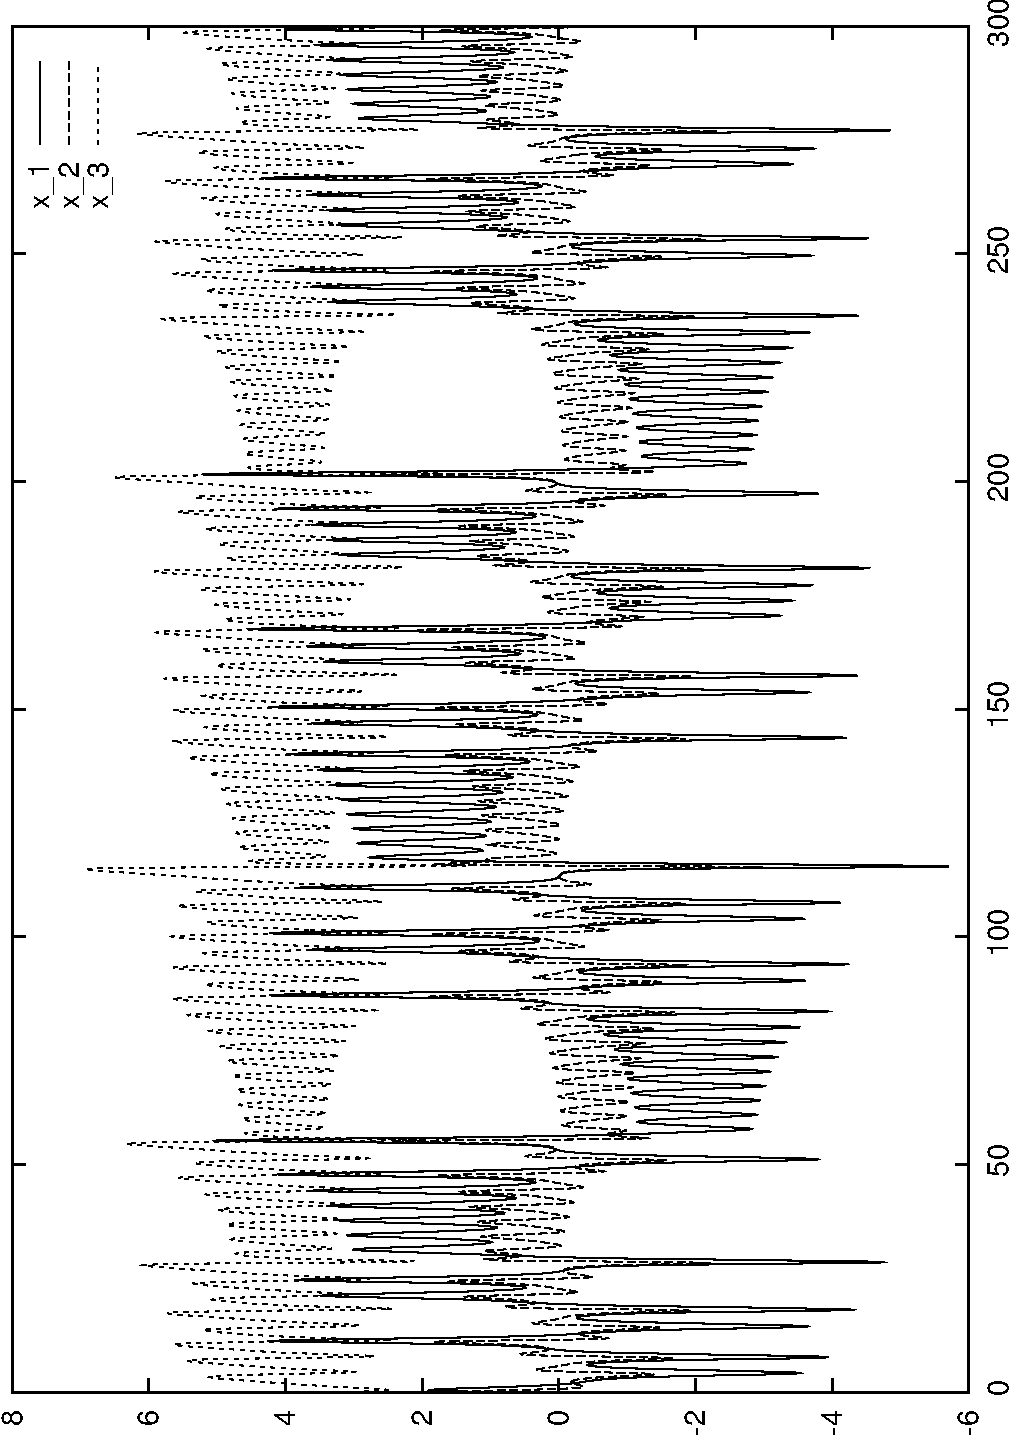
\includegraphics[%
  height=11cm,
  keepaspectratio,
  angle=-90]{figuras/rikitake}


\caption{\label{cap:rikitake2d}Solución del dipolo de Rikitake}
\end{figure}


A primera vista puede parecer que la solución está mal. Si representamos
exactamente el mismo resultado pero mediante una curva paramétrica:

  \begin{verbatim}
>> plot3 (x(:,1),x(:,2),x(:,3))
 \end{verbatim}
llegamos a la figura \ref{cap:rikirake3d}.

%
\begin{figure}[H]
\centering{}

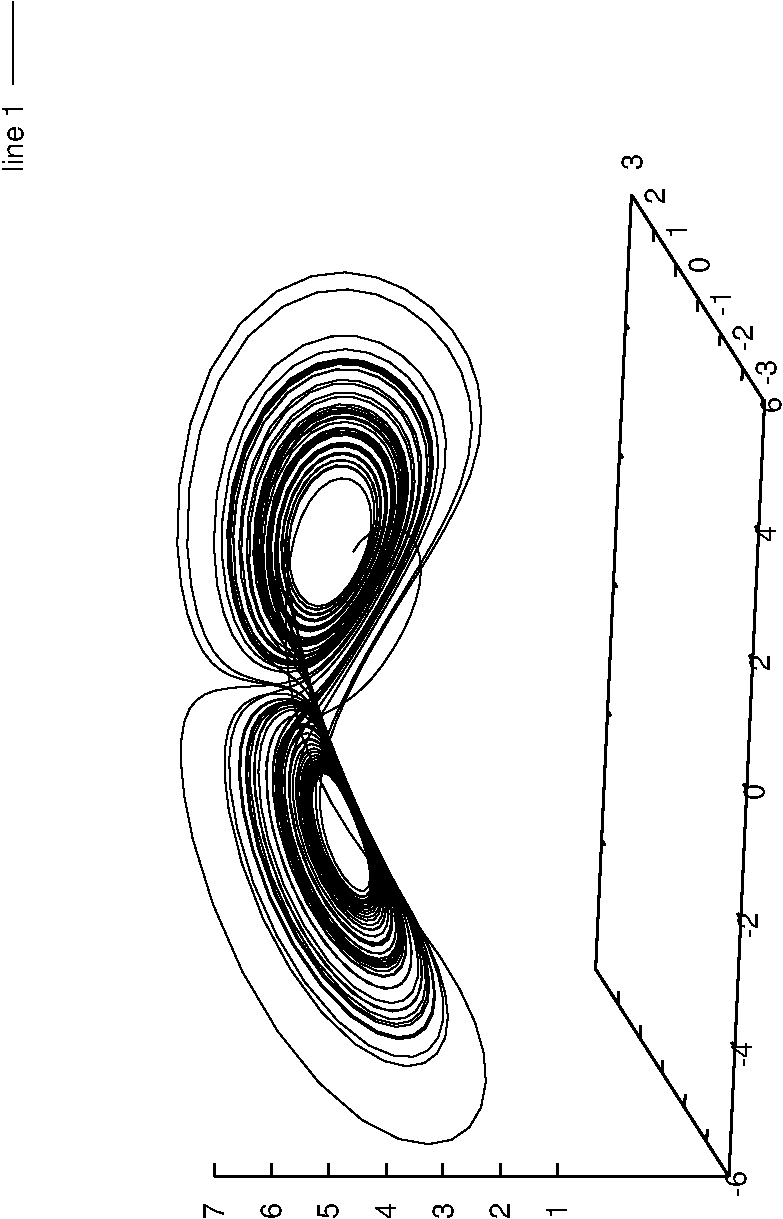
\includegraphics[%
  height=11cm,
  keepaspectratio,
  angle=-90]{figuras/rikitake3d}


\caption{\label{cap:rikirake3d}Curva solución del dipolo de Rikitake}
\end{figure}


De este ejemplo aprendemos que las ecuaciones diferenciales no lineales
pueden tener un comportamiento extraño. Un ejemplo claro de ello son
las ecuaciones de Navier Stokes. Si simplificamos las ecuaciones para
flujo incompresible nos encontraremos un término lineal (el viscoso)
y uno no lineal (el convectivo). El estudio analítico de estas ecuaciones
aún no ha llegado a la conclusión sobre la existencia y la unicidad
de la solución%
\footnote{El estudio de existencia y unicidad de la solución de las ecuaciones
de Navier Stokes para el caso incompresible es uno de los grandes
problemas no resueltos de las matemáticas.%
}, sin embargo se resuelven por métodos numéricos.

La turbulencia, uno de los fenómenos físicos más complejos, aparece
de forma espontanea cuando intentamos resolver las ecuaciones de N-S.
Parte de la disciplina de la CFD (Computational Fluid Dynamics) es
estudiar los flujos turbulentos a partir de la resolución numérica
de las ecuaciones de N-S.

La conclusión es que la integración numérica de ecuaciones diferenciales
es un problema complejo no sólo por la física del problema sino porque
además se suman muchos otros factores. En esta pequeña introducción
sólo hemos visto los problemas stiff y un caso muy sencillo de caos
pero los problemas pueden complicarse muchísimo más.


\section{Cálculo simbólico}

La afirmación repetida hasta la saciedad de que Matlab es un programa
\emph{estrictamente} de cálculo matricial no es del todo correcta.
Se basa en la aplicación del sentido crítico a una herramienta. La
versión completa de Matlab incluye el programa de cálculo simbólico
más utilizado actualmente, Maple. Los problemas generados por el uso
del cálculo simbólico en Matlab son dos:

\begin{enumerate}
\item Tenemos acceso al núcleo de cálculo de Maple, pero dicho acceso no
es completo. Podemos efectuar las operaciones básicas como derivar,
buscar primitivas, crear desarrollos de Taylor... Nunca dispondremos
de la potencia de este tipo de programas.
\item La arquitectura de matlab \textbf{no está pensada para el cálculo
simbólico}. Los programas de cálculo simbólico suelen incluir un interfaz
llamado \emph{notebook} que sirve para ver las fórmulas de entrada
y salida en una notación mucho más matemática. Las diferencias en
el diseño de un programa de cálculo numérico y otro de cálculo simbólico
son a mi parecer irreconciliables.
\end{enumerate}
Esto no significa que sea un crimen utilizar las funciones de cálculo
simbólico cuando uno disponga de ellas. Somos libres de hacer lo que
queramos pero debemos ser conscientes de hasta qué punto no estamos
utilizando la herramienta ideal para nuestro fín.

Octave también dispone de un soporte muy limitado para realizar operaciones
simbólicas. Se podría decir que lo único que puede hacer es derivar
y resolver sistemas de ecuaciones lineales. Tampoco parece que en
un futuro cercano estas funcines se amplíen hasta un soporte equivalente
al de Matlab. No son compatibles pero las funciones son tremendamente
parecidas.

Los siguientes apartados sirven como introducción general al uso de
variables simbólicas pero no conseguiremos más que arañar la superficie
del total de las posibilidades del toolkit.


\subsection{Definición de variables y funciones simbólicas}

\emph{Una de las diferencias más esenciales entre Matlab y Octave en
  lo que respecta a cálculo simbólico es que en Octave es necesario
  activar el toolkit con el siguiente comando}:

\begin{verbatim}
>> symbols
\end{verbatim}
Tanto en Matlab como en Octave el modo más fácil de definir una
variable simbólica es crear una variable que contenga un argumento
simbólico del mismo nombre:

\begin{description}
\item [sym\index{sym}]Define una variable que contiene un argumento
  simbólico.  Es muy recomendable que la variable y el argumento
  tengan el mismo nombre para evitar confusiones
\end{description}
\begin{verbatim}
>> x = sym('x')
\end{verbatim}
\begin{description}
\item [poly2sym\index{poly2sym}]Define un polinomio simbólico a partir
  de sus coeficientes.
\end{description}
\begin{verbatim}
>> poly2sym([1 2 3 -2 10])
ans =
10.0+(-2.0+x*(3.0+(2.0+x)*x))*x
\end{verbatim}

\subsection{Funciones simbólicas elementales.}

La aplicación de funciones elementales a variables simbólicas es completamente
distinta en Matlab y en Octave. Mientras Matlab no diferencia las
funciones simbólicas de las numéricas Octave prefiere llamarlas de
un modo distinto. Esta distinción suele ser que la primera letra de
la función es una mayúscula%
\footnote{Siempre viene bien recordar que la arquitectura de Matlab distingue
entre mayúsculas y minúsculas%
}. Entonces, para conseguir la función simbólica $\sin x$ en Matlab
haremos:

  \begin{verbatim}
>> x=sym('x')
x =
x
>> y=sin(x)
y =
sin(x)
 \end{verbatim}
Mientras que en Octave haremos lo siguiente:

  \begin{verbatim}
>> x=sym('x')
x =
x
>> y=Sin(x)
y =
sin(x)
 \end{verbatim}
En la colección podemos encontrar todas las funciones trigonométricas,
exponenciales, logaritmos...


\subsection{Operaciones simbólicas}

Casi todas las operaciones disponibles en el paquete simbólico de
Octave están dedicadas a la manipulación simbólica de polinomios (muy
interesante en el cálculo numérico). En cambio Matlab dispone de la
mayoría de las operaiciones simbólicas existentes... Derivadas, primitivas,
desarrollos en serie... La única función interesante en lo referente
a cálculo simbólico que tiene Octave es la siguiente:

\begin{description}
\item [subs\index{subs}]Substituye una o varias variables de una expresión
simbólica.
\item [collect\index{collect}]Agrupa los términos polinómicos en una variable
dada.
\item [expand\index{expand}]Desarrolla una expresión simbólica.
\item [differentiate\index{differentiate}]Sólo en Octave. Calcula la n-ésima
derivada de una expresión simbólica.
\end{description}
Función que en Matlab recibe un nombre distinto:

\begin{description}
\item [diff\index{diff}]Sólo en Matlab. Calcula la n-ésima derivada de
una expresión simbólica.
\end{description}
Matlab dispone además de las siguientes operaciones:

\begin{description}
\item [int\index{int}]Encuentra la primitiva de una función simbólica
\item [limit\index{limit}]Calcula el límite hacia un determinado valor
de una función simbólica.
\item [taylor\index{taylor}]Calcula el desarrollo en serie de Taylor respecto
a un punto dado de una función simbólica.
\item [symsum\index{symsum}]Calcula la suma de dos series.
\end{description}
Una de las pocas operaciones compatibles es la representación de una
curva determinada por una función simbólica:

\begin{description}
\item [splot\index{splot}]Dibuja la curva representación de una función
simbólica de una variable. El segundo argumento es un vector de dos
elementos con el intervalo de la variable independiente.
\end{description}
  \begin{verbatim}

 \end{verbatim}
